\chapter{Proposed System: Pipeline Design}
\label{ch:method}

Figure~\ref{fig:pipeline} shows the experimental pipeline. Every stage is fixed and identical across conditions except the reasoning layer, so a measured difference in output quality is attributable to the reasoning topology alone. The figure also separates two graphs that must not be confused: the \emph{evidence graph} (steps 01--03), built once and shared by all methods, and the \emph{thought graph} built inside the reasoning layer.

\begin{figure}[H]
\centering
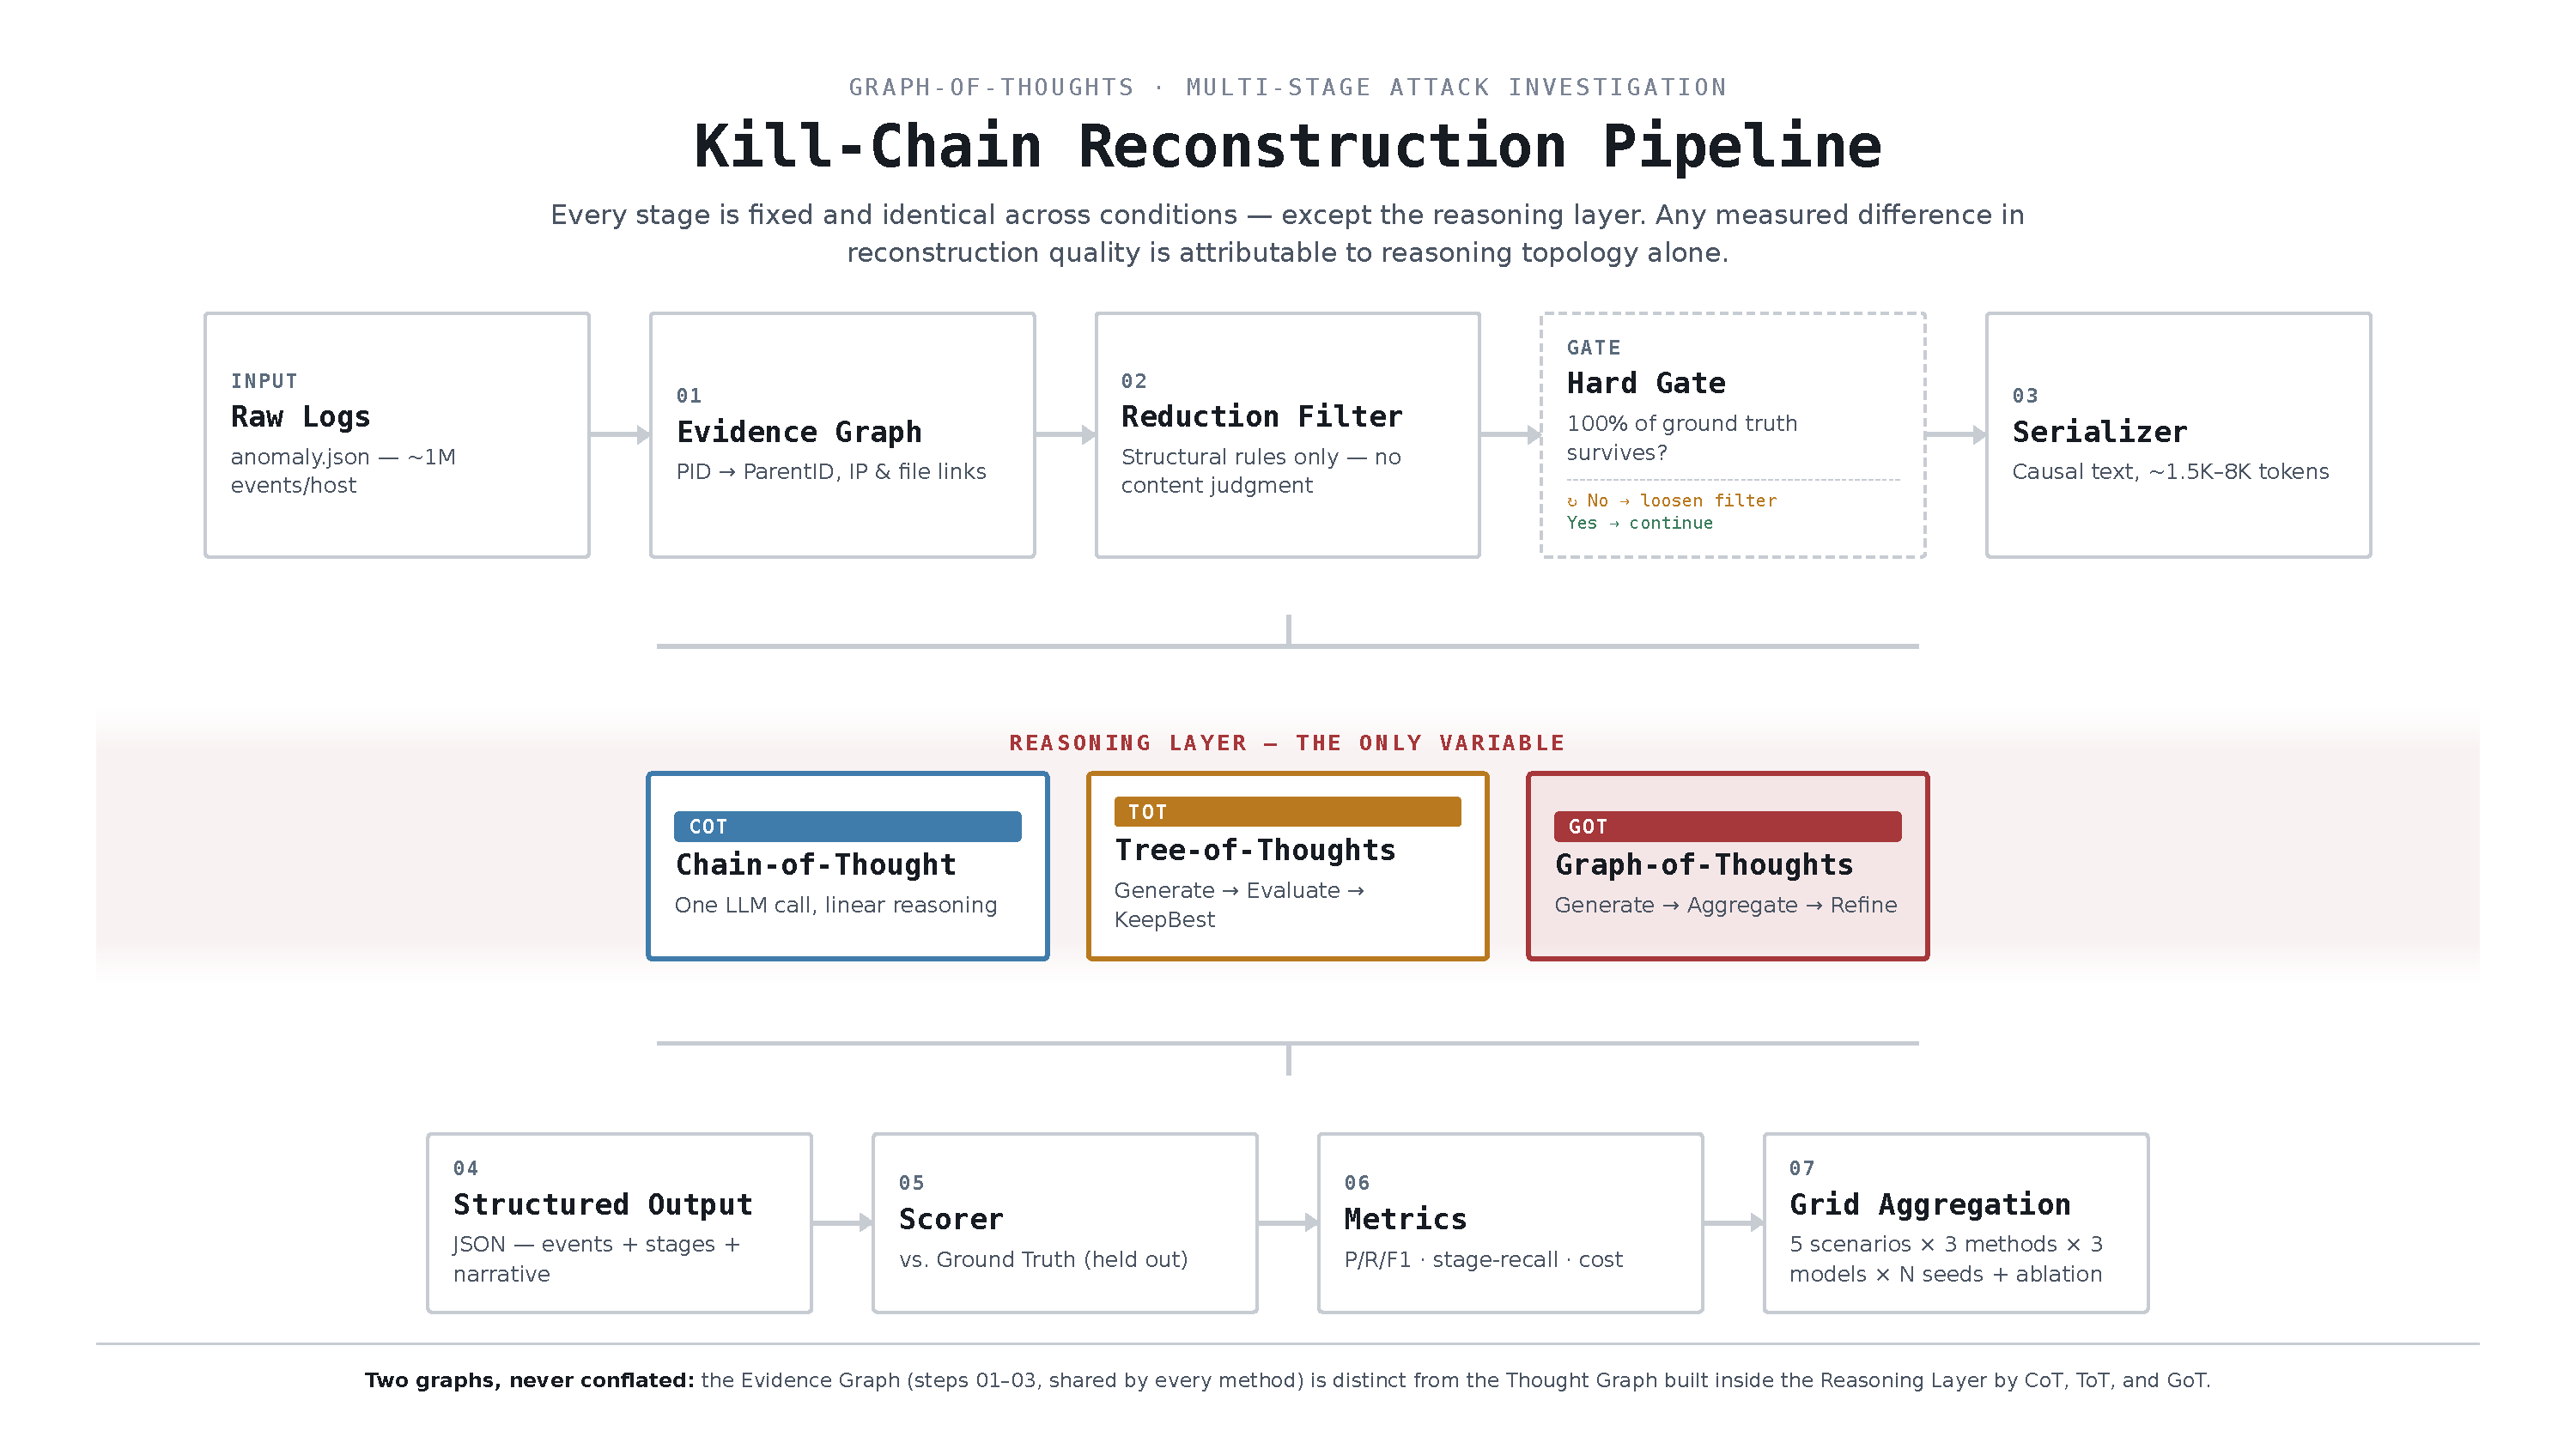
\includegraphics[width=\textwidth]{kill_chain_pipeline}
\caption{Kill-chain reconstruction pipeline. The figure is the design schematic: the token range and the number of models shown in it are planning values. The realised values are 16K to 58K tokens per scenario (Table~\ref{tab:graphstats}) and two base models in the main grid (Table~\ref{tab:models}).}
\label{fig:pipeline}
\end{figure}

\section{Ground-Truth Parser}
For each scenario, the attack annotation files are parsed into a list of nodes. Each node has a stage and a match substring, for example a fragment of the attack command. The pairing of stage and substring was resolved by hand, scenario by scenario, because the identifier join between the annotation files and the attack-analysis spreadsheet differs between scenarios (Section~\ref{sec:gt}). All 89 nodes have a verified pair. Ground truth is read only by the scorer and is never shown to a model.

\section{Evidence Graph and Reduction}
\label{sec:evidence}
The evidence graph has three node types: processes, external IP addresses and files. Edges are of three kinds: \texttt{spawned} (parent process to child), \texttt{connected\_to} (process to an external address) and \texttt{wrote} (process to a suspicious file path). Windows scenarios are parsed from ETW-style records and the Ubuntu scenario from sysdig/Falco-style system-call records, which have a different schema, so there are two parsers. Process nodes are keyed on process identity including start time rather than on the PID alone, because PIDs are reused.

Reduction keeps all process-start nodes, external network connections and suspicious file writes, and collapses exact repeats of the same image, command line and parent. It uses only event type and external-address rules. It does not judge whether a process looks malicious. If it did, the pipeline would contain a hidden detector and the claim that the language model performs the investigation would be false. The dataset's own label field \texttt{is\_warn} is never read.

Figure~\ref{fig:evidence} shows the evidence graph built for the WS12 scenario. Only the branches that touch an external address or a suspicious write, with the process ancestry needed to reach them, are drawn, because the full graph of 234 nodes is not legible as a static image. The complete graph is stored in the repository.

\begin{figure}[p]
\centering
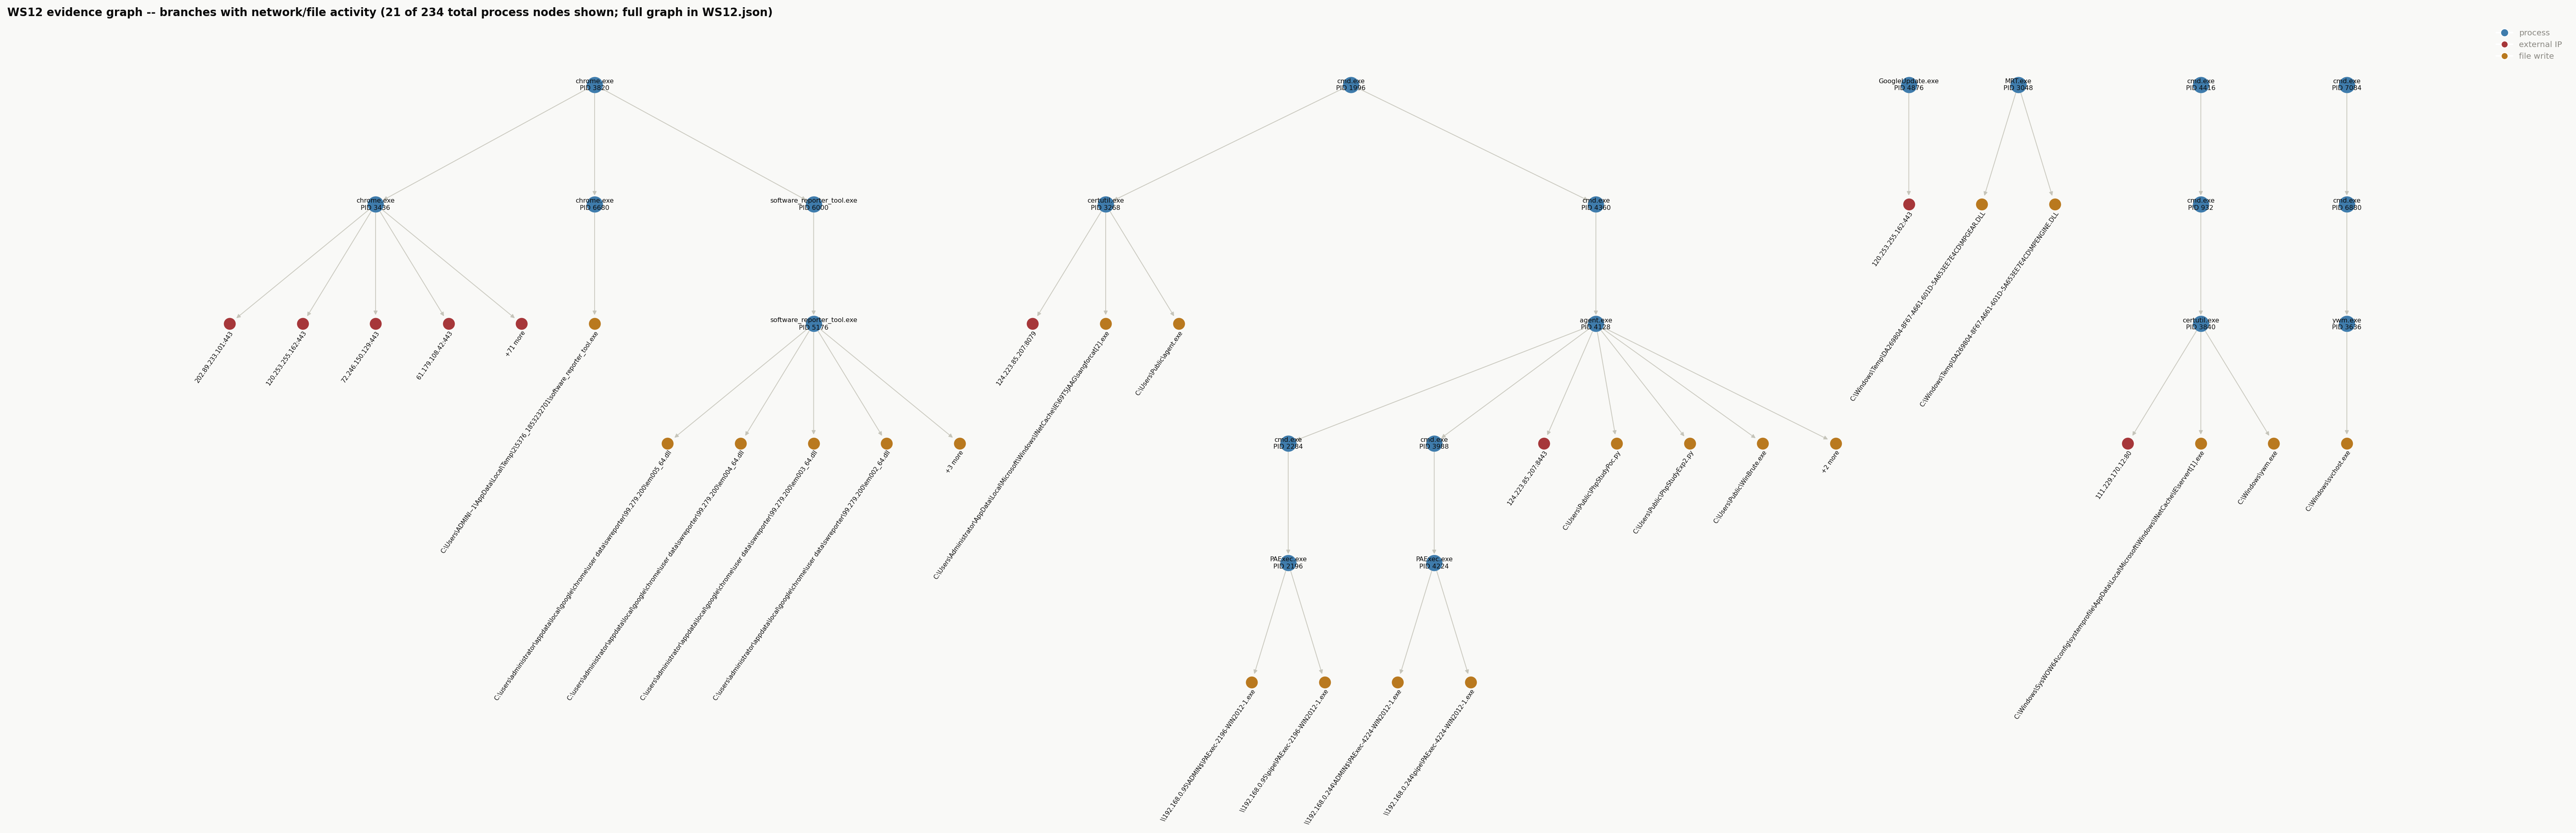
\includegraphics[angle=90,height=0.82\textheight]{fig_evidence_ws12}
\caption{Evidence graph of the WS12 scenario after reduction (filtered view). Process nodes, external IP nodes and file-write nodes are drawn in different colours; parent-to-child process edges follow the process tree.}
\label{fig:evidence}
\end{figure}

\paragraph{Hard gate.} After reduction we check that every ground-truth match substring occurs in the command lines of the reduced set. All five scenarios pass. Documented exceptions are the two nodes that cannot be checked because the ground truth carries no match text, and one Ubuntu node that comes from a second host reached by lateral movement. A scenario that failed the gate would not be run, because recall would then be capped by preprocessing rather than by the method.

\section{Serializer}
The reduced graph is written as plain text with one process tree per root process, ordered chronologically, with children indented and network and file activity listed beneath each process. Command lines longer than 600 characters are truncated for display only; the gate always checks the full text. The format is identical for every scenario and method.

\section{Shared Prompt and Parser}
One prompt template and one parser serve all three topologies. The model is asked for JSON with a list of malicious events (command and stage) and a narrative. For models that do not emit an internal reasoning trace, grammar-constrained decoding guarantees valid JSON. For the security-tuned model, which writes a reasoning trace first, constrained decoding is disabled because it would forbid the opening token of the trace; the parser removes the trace before extracting the JSON. When a later step fails to parse, the parser keeps the last valid state.

\section{Method Implementations}
CoT, ToT and GoT are implemented in separate modules over the \texttt{graph-of-thoughts} framework~\cite{besta2024got}, all using the same prompter and parser. That package imports an attribute that exists only in \texttt{openai} before version~1.0 although it never uses it; a stub module avoids downgrading the SDK needed elsewhere. GoT's per-segment steps run as small controllers sharing one model instance so that cost accumulates correctly.

\section{Improvement Variants}
After the baseline we tested four changes, each applied to all three topologies unless stated, and each tested separately:
\begin{description}[leftmargin=2.6em,style=nextline]
\item[v2] Output limit raised from 1536 to 4096 tokens, to test whether truncation hid answers.
\item[v3] Short definitions of each stage added to the shared prompt (Table~\ref{tab:tactics}).
\item[v4] A per-process triage call before labelling: the model first marks which processes look suspicious, and reasoning sees only those. Triage output is cached per scenario, model and seed and reused by all three topologies, so they see identical triaged evidence.
\item[v5] GoT only: the Aggregate call receives the cross-segment structural links (Section~\ref{sec:framework-links}).
\end{description}
\label{sec:framework-links}

\section{Scorer}
The scorer (Section~\ref{sec:metrics}) was written and unit-tested against hand-verified known-good and known-bad WS12 outputs before any reasoning method existed, and then locked. Two defects were found by the tests and fixed for all methods at once (Chapter~\ref{ch:audit}).
